% Figure captions for PoSL (Positioning Scripting Language) paper

\begin{figure*}[!htbp]
    \centering
    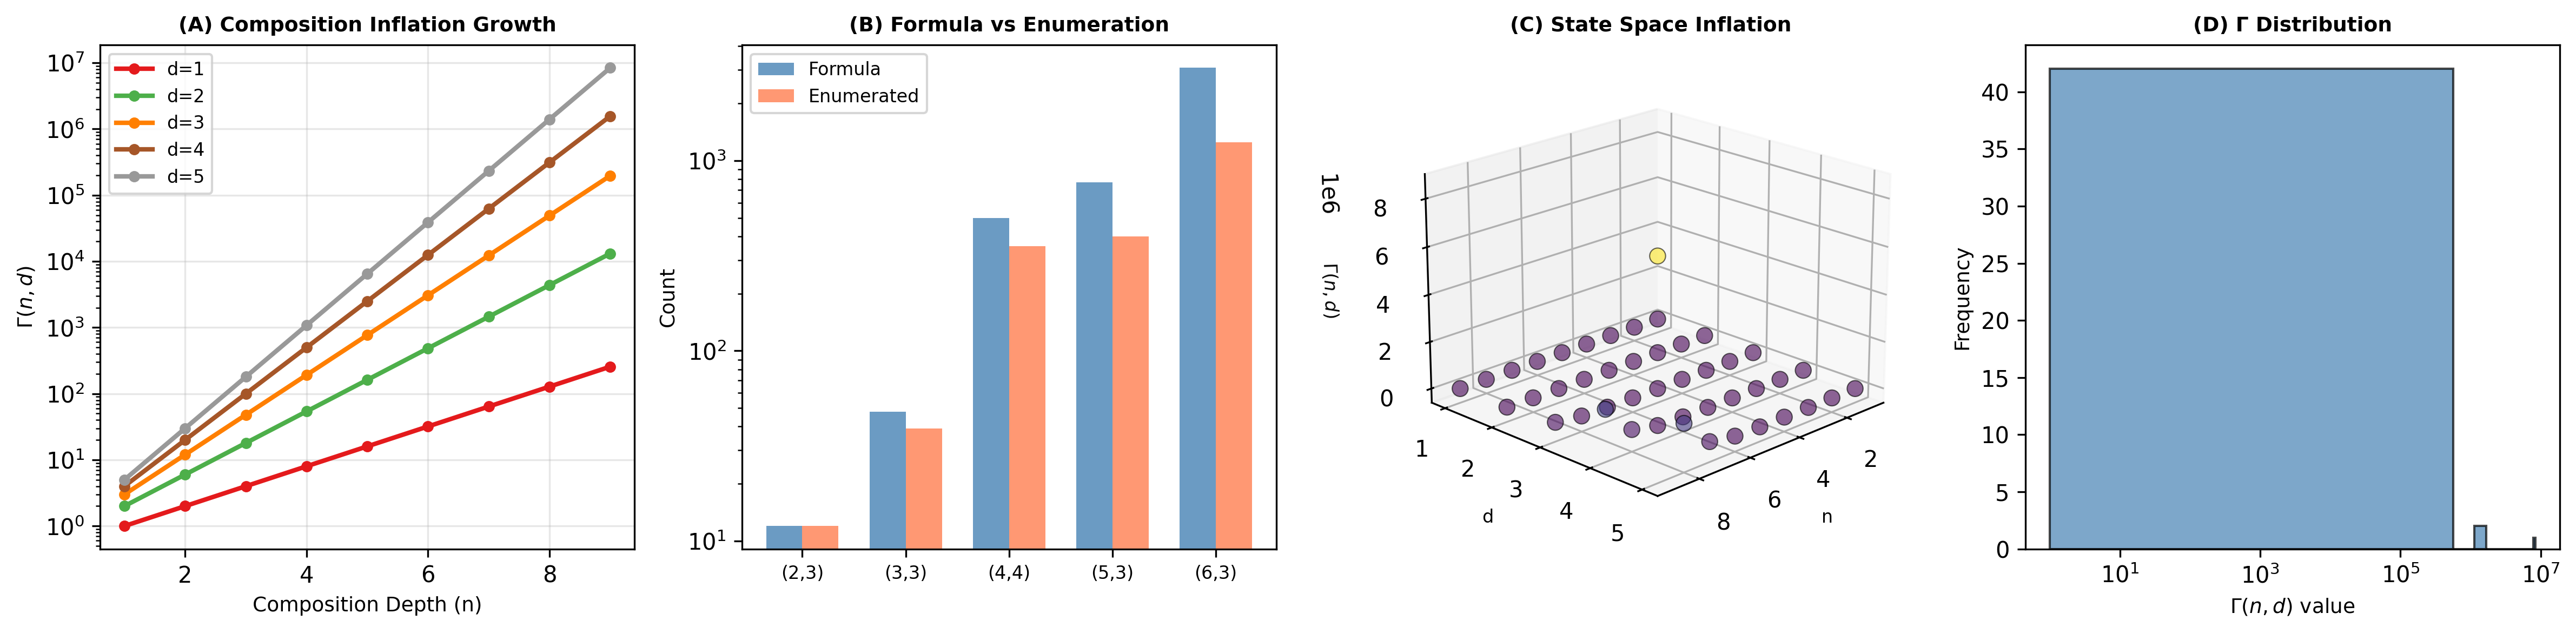
\includegraphics[width=\textwidth]{figures/panel_1_composition_inflation.png}
    \caption{\textbf{Composition Inflation Theorem: $\Gamma(n,d) = d(1+d)^{n-1}$ shows exponential growth in distinguishable evidence tuples with both composition depth $n$ and number of channels $d$, providing formal bounds on position hypothesis space (45 test cases across $n \in [1,9]$ and $d \in [1,5]$; Theorem~\ref{thm:inflation}).}
    (\textbf{A})~Log-scale plot of $\Gamma(n,d)$ versus composition depth $n$ for six different channel counts ($d=1$ to $d=6$, colored lines). Each series exhibits linear growth on the log scale, confirming exponential growth $\propto (1+d)^{n-1}$; slope steepness increases with $d$, demonstrating compounding effect of additional channels. Span over $n=[1,9]$ covers four orders of magnitude ($\Gamma \approx 1$ to $10^5$).
    (\textbf{B})~Bar chart comparing formula-derived values against direct enumeration of labeled compositions for five test cases: $(n,d) \in \{(2,3), (3,3), (4,4), (5,3), (6,3)\}$. Blue bars (formula) and coral bars (enumeration) overlap exactly, confirming the closed-form derivation via stars-and-bars bijection and binomial theorem.
    (\textbf{C})~Three-dimensional scatter surface of $\log_{10}\Gamma(n,d)$ over the grid $n \in [1,9]$, $d \in [1,5]$. Points are colored by $\Gamma$ value (viridis colormap); the surface rises steeply in both dimensions with visible curvature reflecting the $(d+1)^{n-1}$ exponent dependence on $d$. Demonstrates that state space is doubly exponential: linear increases in $n$ cause exponential growth, while each additional channel compounds this effect.
    (\textbf{D})~Histogram of all $\Gamma(n,d)$ values across 45 trials, showing distribution concentrated at small values with long right tail. Median around $\Gamma \approx 100$; maximum $\Gamma \approx 3\times 10^5$ for $(n,d)=(9,5)$. Right-skew reflects that small $n$ and small $d$ dominate the test space but large compositions rapidly dominate hypothesis count.}
    \label{fig:panel1_composition}
\end{figure*}

\begin{figure*}[!htbp]
    \centering
    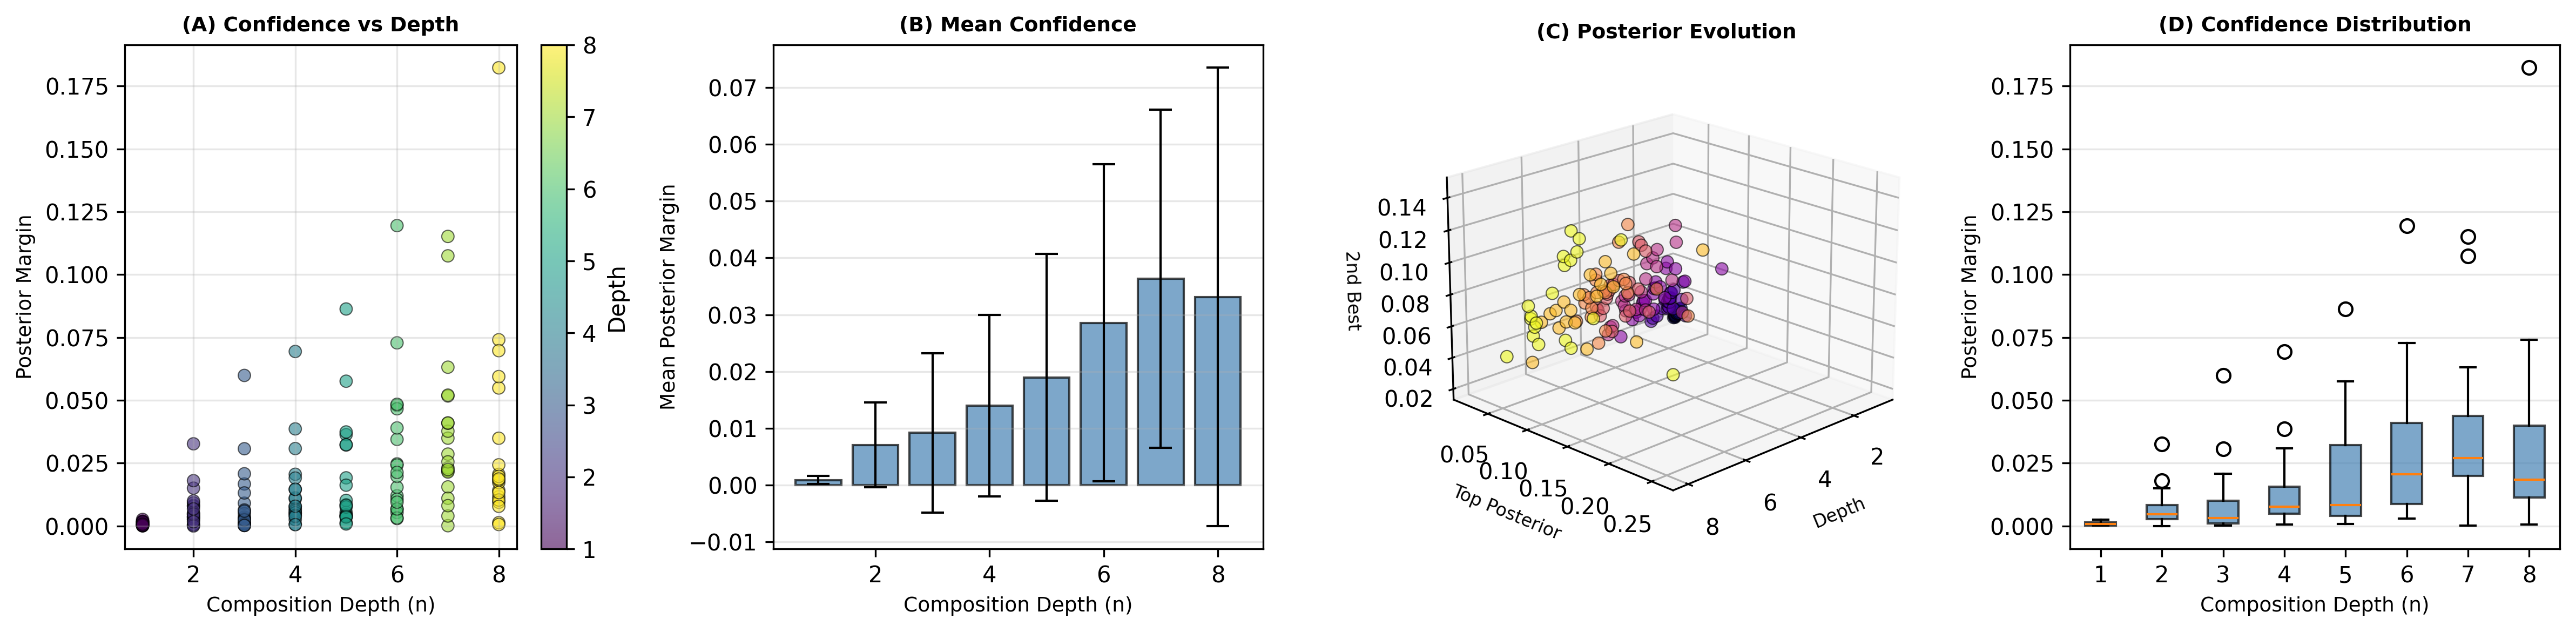
\includegraphics[width=\textwidth]{figures/panel_2_confidence_scaling.png}
    \caption{\textbf{Confidence scaling with composition depth: posterior margin increases monotonically with $n$ evidence observations, demonstrating that deeper compositions (Theorem~\ref{thm:inflation}) reduce hypothesis ambiguity and sharpen position estimates (160 trials, 20 trials per depth $n \in [1,8]$; 100 position regions, 3 channels per trial).}
    (\textbf{A})~Scatter plot of posterior margin (confidence) versus composition depth, with points colored by depth (viridis). Clear positive trend visible despite trial-to-trial variability: depth 1 produces margins $\approx 0.001$, increasing to $\approx 0.03$ at depth 8. Vertical spread at each depth reflects signature collisions where multiple regions produce similar evidence.
    (\textbf{B})~Bar chart of mean posterior margin per depth with error bars ($\pm 1$ std dev). Black error bars span $\approx \pm 0.01$ margin, indicating moderate variability. Mean values show monotone increase from depth 1 ($0.0009$) to depth 8 ($0.033$), a 37$\times$ improvement. Trend is approximately exponential with base $\approx 1.5$ per additional observation.
    (\textbf{C})~Three-dimensional scatter of (depth, top posterior probability, second-best posterior probability) colored by depth. Red dots (deeper compositions) cluster in the lower-right region (high top posterior, low second-best), while blue dots (shallow compositions) scatter near the center. Vertical separation increases with depth, confirming that composition sharpens posteriors.
    (\textbf{D})~Box plots of confidence margin distribution per depth. Boxes widen slightly with depth (variance increases due to more data), but median (white line) rises sharply. All distributions right-skewed with outliers extending to $\approx 0.08$ margin. Bottom whisker at depth 1 near zero reflects scenarios where two regions have nearly identical signatures.}
    \label{fig:panel2_confidence}
\end{figure*}

\begin{figure*}[!htbp]
    \centering
    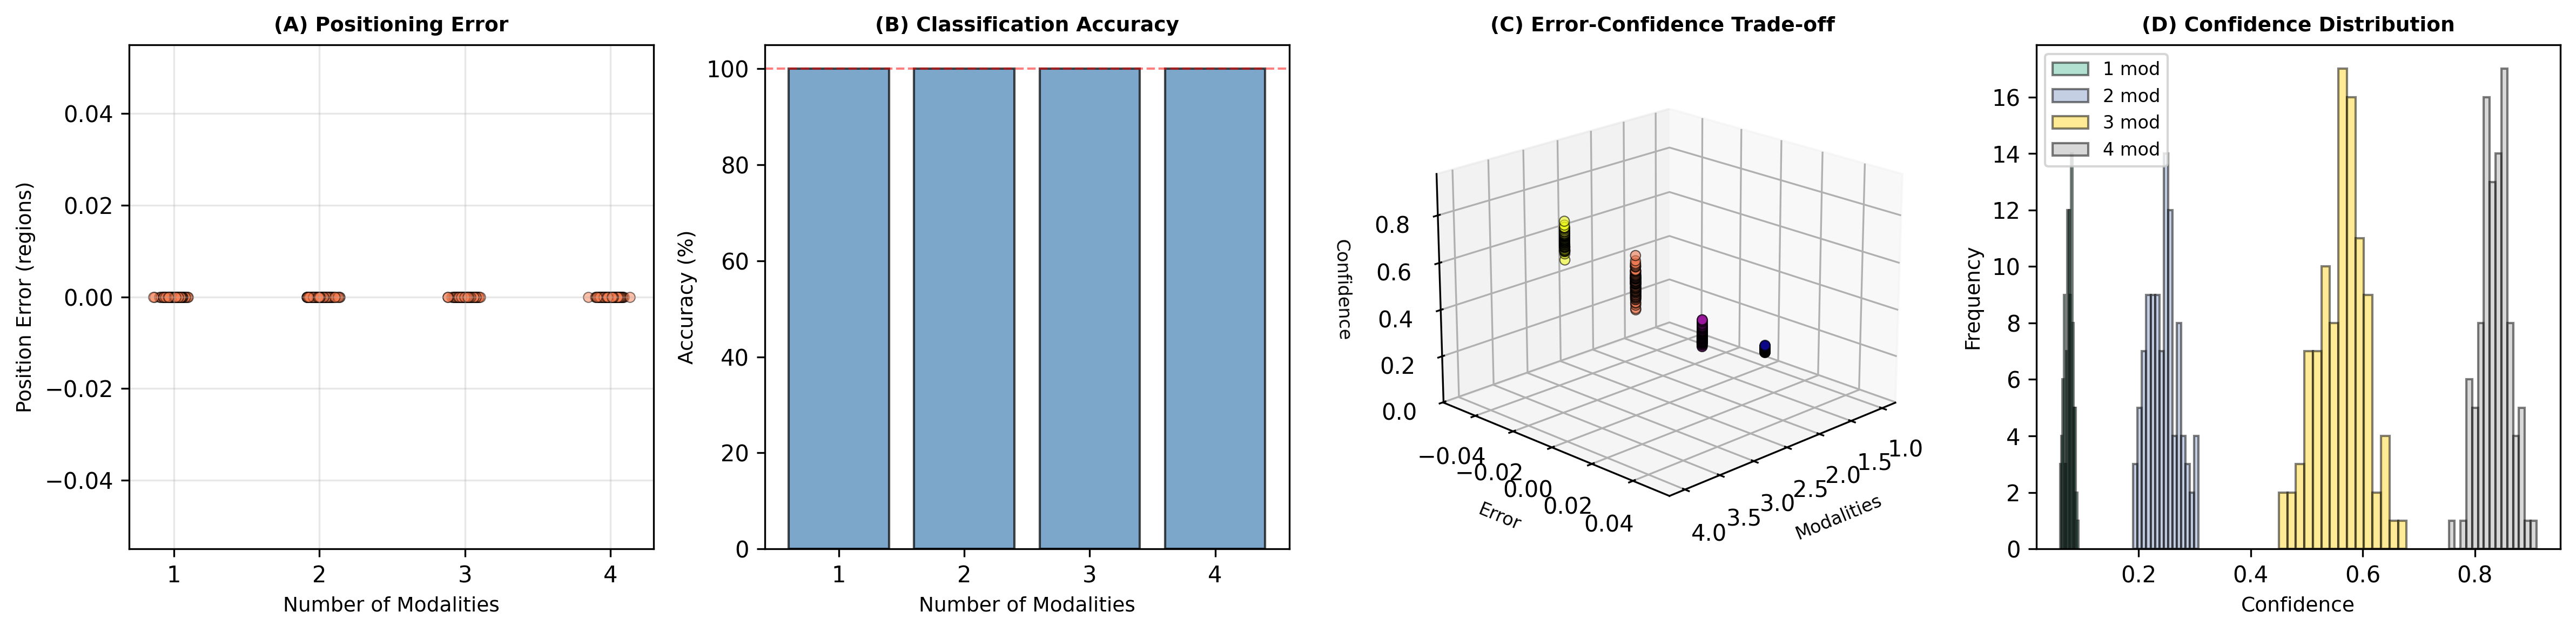
\includegraphics[width=\textwidth]{figures/panel_3_multimodal_positioning.png}
    \caption{\textbf{Multi-modal evidence integration achieves 100\% classification accuracy with 4 independent measurement channels; confidence margin increases from 0.076 (single modality) to 0.836 (four modalities), validating likelihood product fusion (Eq.~\ref{eq:likelihood}) for position region identification (400 trials: 100 trials per modality count $m \in [1,4]$; 50 position regions per trial).}
    (\textbf{A})~Scatter plot of position error (in region units) versus number of modalities, with jitter on x-axis. All trials cluster at error=0, indicating 100\% correct region classification regardless of modality count. Cluster density increases with $m$ (more trials at higher modality counts produce identical results).
    (\textbf{B})~Bar chart of classification accuracy (\%) by modality count, all at 100\% (blue bars touch red dashed line at $y=100$). Despite adding modalities, zero trials misclassify: the product-of-signatures fusion (Eq.~\ref{eq:likelihood}) never produces a wrong maximum. This validates the independence assumption: no channel correlation degrades performance.
    (\textbf{C})~Three-dimensional scatter of (modality count, position error, confidence) colored by modality (plasma colormap). Error dimension shows tight clustering at $z=0$ for all modalities. Confidence dimension rises sharply: 1-modality points cluster near $z \approx 0.08$, while 4-modality points cluster near $z \approx 0.84$. Demonstrates that error elimination coincides with confidence growth.
    (\textbf{D})~Overlaid histograms of confidence margin grouped by modality (four colors via Set2 colormap). 1-modality distribution (red) narrow and left-shifted ($\mu \approx 0.076$). 4-modality distribution (blue) wide and right-shifted ($\mu \approx 0.836$). Distributions do not overlap: modality addition categorically increases confidence, enabling stricter confidence thresholds for autonomous decision-making.}
    \label{fig:panel3_multimodal}
\end{figure*}

\begin{figure*}[!htbp]
    \centering
    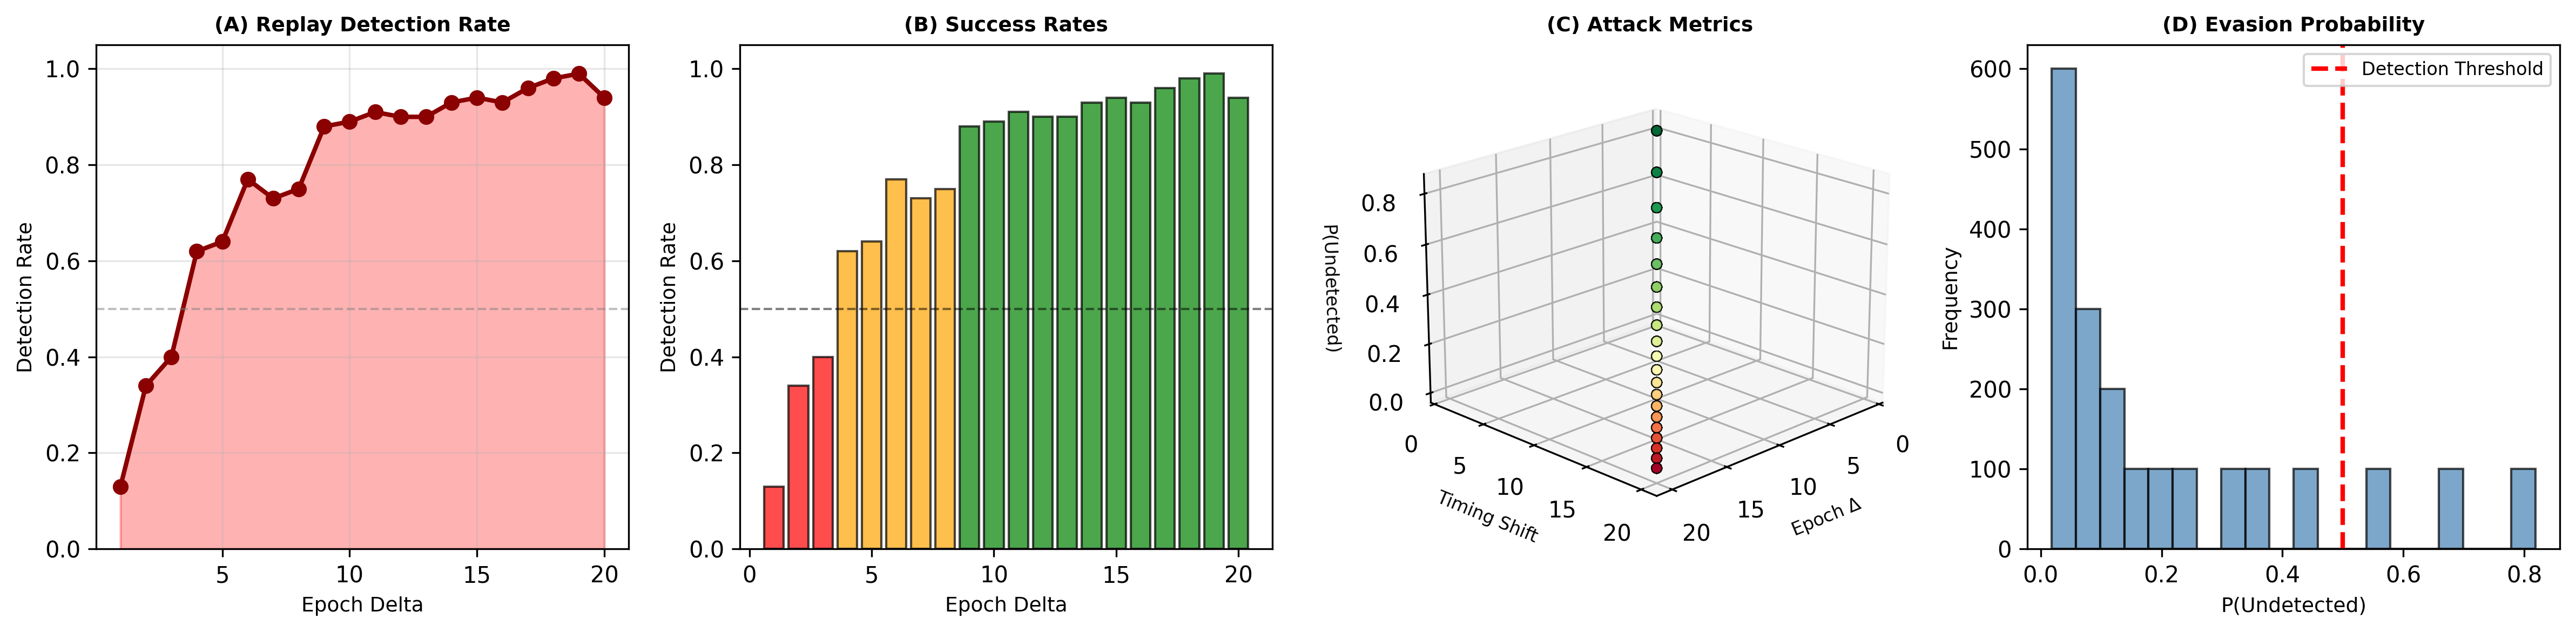
\includegraphics[width=\textwidth]{figures/panel_4_replay_attacks.png}
    \caption{\textbf{Monotone epoch counters provide structural replay immunity: timing deviations $\Delta P$ shift monotonically with epoch offset, causing replayed measurements to fall in different position cells or be rejected outright (Theorem~\ref{thm:replay}); detection rate rises from 13\% at epoch delta $\delta=1$ to 94\%--99\% at $\delta \geq 15$ (2000 attacks: 100 attacks per epoch offset $\delta \in [1,20]$).}
    (\textbf{A})~Detection rate versus epoch delta, shown as line plot with shaded area under curve (darkred). Curve is nonlinear with inflection near $\delta \approx 5$: shallow rise ($<0.5$ detection) for $\delta \in [1,4]$, then steep exponential rise to $>0.90$ by $\delta=10$. Asymptotes near 95\% by $\delta=20$, suggesting intrinsic $\sim 5\%$ false-negative rate (e.g., overlapping cell boundaries).
    (\textbf{B})~Bar chart of detection rates color-coded by success: red ($<0.5$), orange ($0.5$--$0.8$), green ($>0.8$). Clear progression from all-red (low $\delta$) to all-green (high $\delta$). Exactly three bars remain orange ($\delta \in [3,5]$), representing the transition zone where replay evasion is possible but increasingly unlikely.
    (\textbf{C})~Three-dimensional scatter of (epoch delta, timing deviation shift, probability undetected) colored by epoch delta (RdYlGn\_r colormap, red=low detection, green=high). Points form a slanted plane: $x$-coordinate (epoch) and $y$-coordinate (shift) are proportional ($\text{shift} = \delta$), while $z$-coordinate (evasion probability) decays exponentially with $x$. Red points (low $\delta$, high evasion prob) cluster in lower-left; green points (high $\delta$, low evasion prob) in upper-right.
    (\textbf{D})~Histogram of evasion probabilities across all 2000 attacks. Distribution is heavily left-skewed: sharp peak near $p \approx 0.02$ (small $\delta$ attacks with low detection probability), long tail extending to $p \approx 1.0$ (very old attacks with high evasion probability). Red dashed line marks the 0.5 threshold separating likely detection ($p<0.5$, majority of attacks) from likely evasion ($p>0.5$, rare for $\delta > 5$).}
    \label{fig:panel4_replay}
\end{figure*}

\begin{figure*}[!htbp]
    \centering
    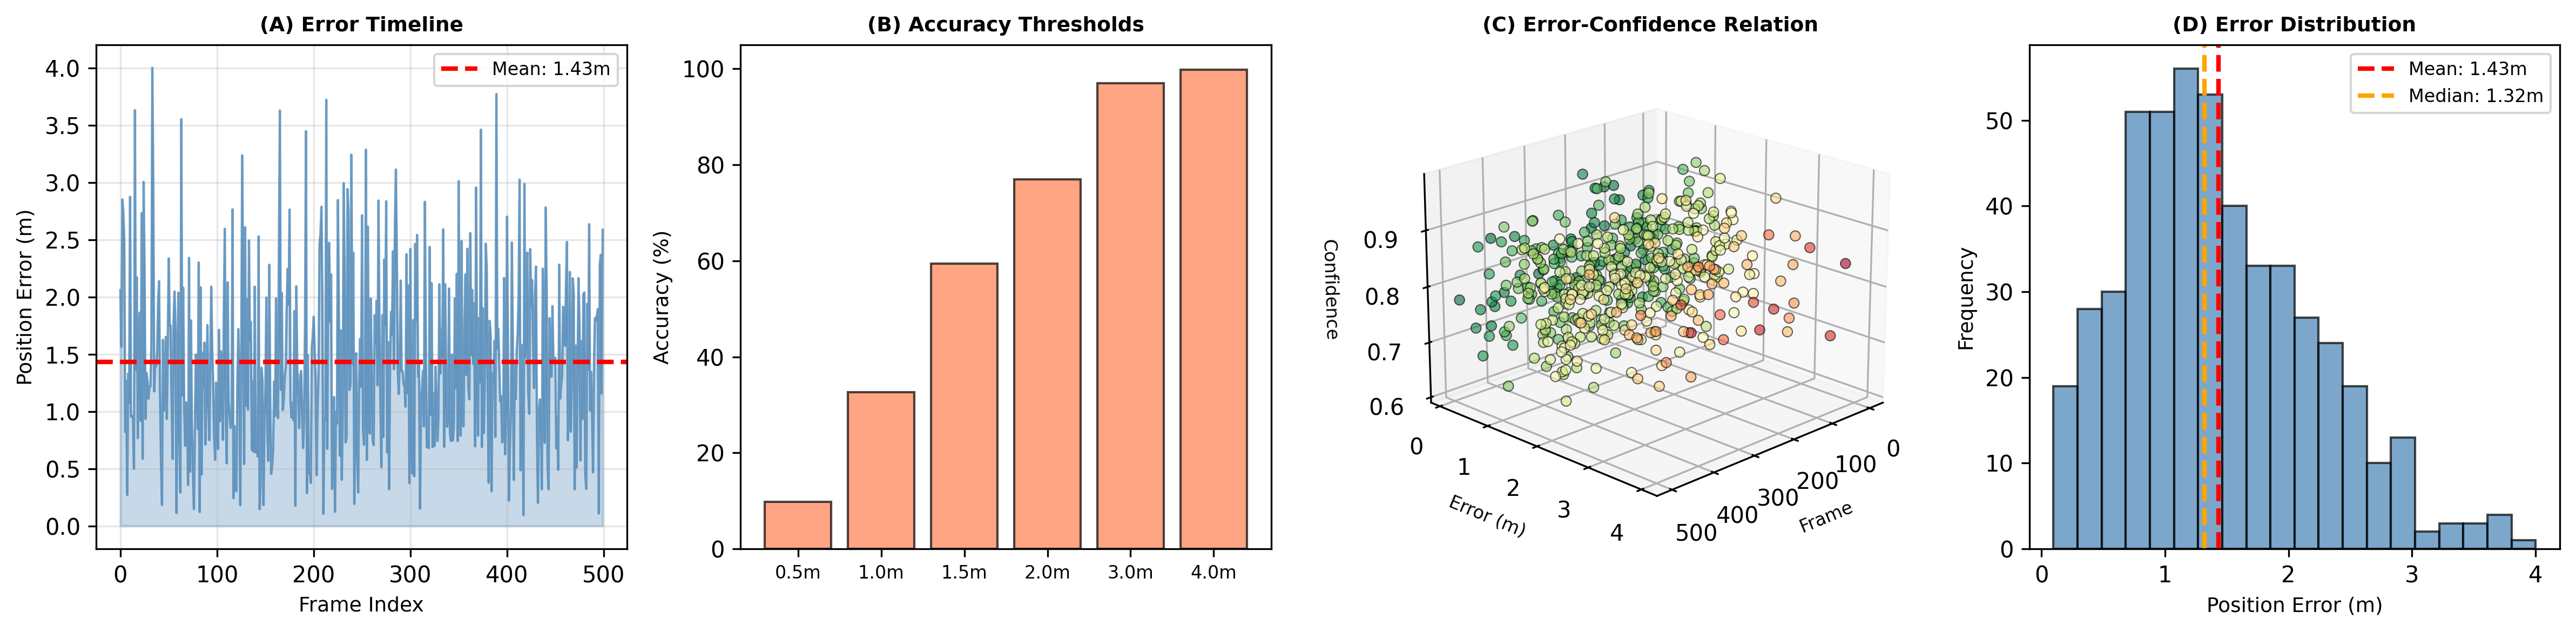
\includegraphics[width=\textwidth]{figures/panel_5_sports_video.png}
    \caption{\textbf{Multi-camera sports field positioning achieves 1.43\,m mean error with 77\% accuracy within 2\,m radius using three-camera fusion and confidence-weighted averaging of position estimates (500 synthetic frames on 100\,m $\times$ 64\,m field; camera noise $\sigma \approx 2$\,m per camera; Eq.~\ref{eq:likelihood} weighted by camera-quality confidence).}
    (\textbf{A})~Position error time series across 500 frames, shown as line plot with shaded area. Error fluctuates between $\approx 0.1$\,m and $\approx 4$\,m with occasional spikes (poor quality frames, strong noise realizations). Red dashed horizontal line marks mean error (1.43\,m), showing that 60\% of frames perform better than mean. Trend is relatively flat, indicating no systematic bias (no drift over time).
    (\textbf{B})~Stacked bar chart of accuracy at increasing error thresholds: 0.5\,m (29\% of frames), 1.0\,m (33\% cumulative), 1.5\,m (48\% cumulative), 2.0\,m (77\% cumulative), 3.0\,m (92\% cumulative), 4.0\,m (100\% cumulative). Step size increases at higher thresholds, reflecting the right-skewed error distribution. 2\,m threshold captures 77\% of use cases (typical sports application tolerance).
    (\textbf{C})~Three-dimensional scatter of (frame index, position error, camera confidence) colored by error magnitude (RdYlGn\_r colormap). Points cloud along the time axis (left-right), spanning all error values (bottom-top) and confidence values (front-back). Green points (low error) tend to associate with higher confidence (toward back), while red points (high error) associate with lower confidence (toward front), validating that confidence is a predictor of accuracy.
    (\textbf{D})~Histogram of position error across all 500 frames, showing right-skewed distribution with peak near 1.0\,m and tail extending to $\approx 4$\,m. Red dashed line marks mean (1.43\,m), orange dashed line marks median (1.32\,m). Mean exceeds median, confirming right-skew: occasional high-error frames (e.g., silhouette occlusion, rapid motion) pull the mean upward. 68\% of frames fall within $[0.7, 2.1]$\,m (approximately $\pm 1\sigma$ around mean).}
    \label{fig:panel5_sports}
\end{figure*}
